\documentclass[12pt,reqno]{amsart}
\usepackage[top=1.5cm, left=1.5cm,right=1.5cm,bottom=1.5cm]{geometry}
\renewcommand{\baselinestretch}{1.2}
\usepackage{amsmath}
\usepackage{amssymb}
\usepackage{scalefnt}
\usepackage{tikz}
\usepackage{color,hyperref,enumerate,multicol}
\definecolor{darkblue}{rgb}{0.0,0.0,0.3}
\hypersetup{colorlinks,breaklinks,
            linkcolor=darkblue,urlcolor=darkblue,
            anchorcolor=darkblue,citecolor=darkblue}
            
\usepackage{algorithm}
\usepackage{algorithmic}
\pagestyle{empty}
\newcommand{\N}{\ensuremath{\mathbb{N}}}
\newcommand{\<}{\ensuremath{\langle}}
\renewcommand{\>}{\ensuremath{\rangle}}
\newcommand{\Z}{\ensuremath{\mathbb{Z}}}
\newcommand{\R}{\ensuremath{\mathbb{R}}}
\newcommand{\meet}{\ensuremath{\wedge}}
\newcommand{\Meet}{\ensuremath{\bigwedge}}
\newcommand{\join}{\ensuremath{\vee}}
\renewcommand{\emptyset}{\ensuremath{\varnothing}}
\renewcommand{\subset}{\ensuremath{\subsetneq}}
\newcommand{\boldemph}{\emph}
\newcommand{\lcm}{\operatorname{lcm}}

\begin{document}
\thispagestyle{empty}

\noindent \textbf{Math 301} \hskip5cm {\bf Homework 4} \hfill {\bf Fall 2014}
\vskip1cm
\noindent {\bf Chapter 3:}  16, 17, 31, 33, 44, 45, 52. \\  
   Additional suggested exercises: 35, 46, 47, 54.  \\
{\bf Due date:} Friday, 9/26

\medskip

\noindent NOTE: the numbers listed above correspond to the printed version of
the textbook, generated from 2013/08/16 source files.

\medskip

\begin{enumerate}

%% 16 %%%%%%%%%%%%%%%%%%%%%%%%%%%%%%%%%%%%%%%%%%%%%%%%
\item[{\bf 16.}]
Give a specific example of a group $G$ and elements $g, h \in G$ where $(gh)^n \neq g^nh^n$. 
 
\medskip
\noindent {\bf Solution:}
Consider the triangle below

\begin{center}
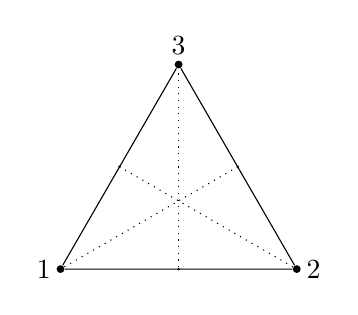
\begin{tikzpicture}[scale=0.75]
  \node (0) at (0,0) [fill,circle,inner sep=.2pt] {};
  \node (1) at (-2,0) [fill,circle,inner sep=1pt] {};
  \node (2) at (2,0) [fill,circle,inner sep=1pt] {};
  \node (3) at (0,3.4641) [fill,circle,inner sep=1pt] {};
  \node (4) at (1, 1.732) [fill,circle,inner sep=.2pt] {};
  \node (5) at (-1, 1.732) [fill,circle,inner sep=.2pt] {};

  \draw (1) node [left] {$1$};
  \draw (2) node [right] {$2$};
  \draw (3) node [above] {$3$};
  \draw (1) to (2) to (3) to (1);
  \draw[dotted] (0) to (3);
  \draw[dotted] (1) to (4);
  \draw[dotted] (2) to (5);

\end{tikzpicture}
\end{center}

The group of symmetries of this triangle has elements
\medskip
\begin{itemize}
\item 
$\mu_1 = \begin{pmatrix}1 & 2 & 3\\2 & 1 &3\end{pmatrix}$
(reflection across the vertical dotted line)
\medskip
\item 
$\mu_2 = \begin{pmatrix}1 & 2 & 3\\1 & 3 &2\end{pmatrix}$
(reflection across the dotted line with positive slope)
\medskip
\item
$\mu_3 = \begin{pmatrix}1 & 2 & 3\\3 & 2 &1\end{pmatrix}$
(reflection across the dotted line with negative slope)
\item 
$\rho_1 = \begin{pmatrix}1 & 2 & 3\\2 & 3 & 1\end{pmatrix}$
(rotation by 60 degrees counter-clockwise)
\medskip
\item 
$\rho_2 = \begin{pmatrix}1 & 2 & 3\\3 & 2 & 1\end{pmatrix}$
(rotation by 120 degrees counter-clockwise)
\medskip
\end{itemize}

The composition of $\mu_1$ and $\mu_2$ is
\[
\mu_1 \mu_2  = 
\begin{pmatrix}1 & 2 & 3\\2 & 1 &3\end{pmatrix}
\begin{pmatrix}1 & 2 & 3\\1 & 3 &2\end{pmatrix}
=
\begin{pmatrix}1 & 2 & 3\\2 & 3 &1\end{pmatrix} = \rho_1
\]
Therefore,
$(\mu_1 \mu_2)^2  = \rho_1^2 = \rho_2$
On the other hand, $\mu_1^2 = \mu_2^2 = e$, the identity permutation
that leaves all elements fixed.  Therefore, 
$(\mu_1 \cdot \mu_2)^2  = \rho_2 \neq e = \mu_1^2 \cdot \mu_2^2$.
\qed

\newpage

%% 17 %%%%%%%%%%%%%%%%%%%%%%%%%%%%%%%%%%%%%%%%%%%%%%%%
\item[{\bf 17.}]
Give examples of three different groups with eight elements.  
Why are the groups different? 
 
\medskip

\noindent {\bf Solution:}
There are exactly five 8-element groups:

\medskip

\begin{center}
\begin{tabular}{c|c|c|c|c}
$G$ & Description & GAP name & IsAbelian($G$) & IsCyclic($G$)\\
\hline
$\Z_8$ & integers modulo 8 &  SmallGroup(8,1) & true & true\\
$\Z_4 \times \Z_2$ & direct product of $\Z_4$ by $\Z_2$ &  SmallGroup(8,2) & true & false\\
$D_4$ & dihedral group on four letters& SmallGroup(8,3) & false & false\\
$Q_8$ & 8-element quarternion group & SmallGroup(8,4) & false & false\\
$\Z_2\times \Z_2 \times \Z_2$& direct cube of $\Z_2$  &  SmallGroup(8,5) & true & false
\end{tabular}
\end{center}

\medskip
We have spend a lot of time discussing the groups $\Z_n$, as well as their
direct products, so we are already familiar with at least three of the groups in
the table, namely, $\Z_8$, $\Z_4 \times \Z_2$, and $\Z_2^3$.  
These groups are all abelian, but only the first is cyclic.  We have also studied the 
group $D_4$, which is the group of symmetries of the square.  It is neither
abelian nor cyclic. We have not yet discussed the quarternion group in lecture,
but it is described in the textbook.

\medskip
\noindent {\it Side note:} Although the students should already be able to fill in the table above by
hand, the following GAP/Sage commands below could also be used to generate this
information (see SmallGroupsLibrary.sagews worksheet):

{\small
\begin{verbatim}
%gap
for k in [1..5] do
    G:=SmallGroup(8,k);
    Print(StructureDescription(G), "  &  SmallGroup(8,", k, ") & ", 
    IsAbelian(G), " & ", IsCyclic(G), "\n");
od;
\end{verbatim}
}


\medskip

%% 31 %%%%%%%%%%%%%%%%%%%%%%%%%%%%%%%%%%%%%%%%%%%%%%%%
\item[{\bf 31.}]
Show that if $G$ is a finite group of even order, then there is an $a
\in G$ such that $a$ is not the identity and $a^2 = e$.
 
\medskip
\noindent {\bf Solution:} Suppose $G$ is a group of even order, say $|G| = 2n$
for $n\geq 1$.  We want to prove there is some non-identity element $a\in G$ such
that $a^2 = e$.  Such a group element, whose square is
the identity, is called an ``involution.''  Notice that, because of the group
properties and cancellation laws, we have
$a^2 = e$ if and only if $a = a^{-1}$.  So, the set of all involutions of $G$ is
given by
\[
\mathcal{I} := \{a \in G : a = a^{-1}\}.
\]
This set is clearly nonempty, since $e\in \mathcal{I}$, so there is at least one
element in $\mathcal{I}$.  Our goal is to show
that, when $G$ has even order, the set $\mathcal{I}$ contains more than one element.

Next, consider the complement of $\mathcal{I}$ in $G$:
\[
\mathcal{I}^c := \{a \in G : a \neq a^{-1}\}.
\]
Notice that this set has an even number of elements.  (If it is empty, then it
has 0 elements.  If it is non-empty, then for each $x\in \mathcal{I}^c$, there
is an $x^{-1} \in \mathcal{I}^c$ distinct from $x$.)
Therefore, 
$\mathcal{I}$ must contain more than one element, otherwise 
$|G| = |\mathcal{I}| + |\mathcal{I}^c| = 1+ |\mathcal{I}^c|$, which is an odd
number, contradicting that $G$ has even order.
\qed
\medskip

%% 33 %%%%%%%%%%%%%%%%%%%%%%%%%%%%%%%%%%%%%%%%%%%%%%%%
\item[{\bf 33.}]
Find all the subgroups of ${\mathbb Z}_3 \times {\mathbb Z}_3$. Use this
information to show that ${\mathbb Z}_3 \times {\mathbb Z}_3$ is not the
same group as ${\mathbb Z}_9$.  (See Example 40 for a short description of the
product of groups.) 

\medskip
\noindent {\bf Solution:}
\medskip
An easy way to begin searching for subgroups of a group is to take an element 
$x \in G$ and find the subset generated by $x$, that is $\<x\> = \{x^k : k \in \N\}$.
It's easy to see that this set is a subgroup of $G$.  In case the group is
abelian, we take multiples of $x$ instead of powers and write 
$\<x \> = \{kx : k \in \N\}$.  Recall, 
\[
x^k = x \cdot x\cdot \cdots \cdot x
\]
\[
kx = x + x + \cdots + x
\]
where the right hand side in each case has $k$ factors.

Recall, the elements of $\Z_3$ are (congruence classes of) integers mod 3. There
are three such classes:
\begin{align*}
[0] &= \{\dots, -3, 0, 3, 6, 9, \dots\}  \\
[1] &= \{\dots, -2, 1, 4, 7, 10, \dots\}  \\
[2] &= \{\dots, -1, 2, 5, 8, 11, \dots\}  
\end{align*}
For ease of notation, let us identify each class with it's natural
representative, i.e., let $0$ denote $[0]$, etc.
Then we can easily write down all of the elements in the (abelian) group 
$\Z_3 \times \Z_3$.  That is, the universe of the 
group $\Z_3 \times \Z_3$ is the set
\[
\{(0,0), (0,1), (0,2),
(1,0), (1,1), (1,2),
(2,0), (2,1), (2,2)\}.
\]
(Sometimes we get sloppy and say that $\Z_3 \times \Z_3$ \emph{is} this
set, but that is not quite right.)

Now let's start generating some subgroups: since $(0,1) + (0,1) = (0,2)$
and $(0,1) + (0,1) + (0,1) = (0,0) \pmod 3$, we see that the subgroup generated
by $(0,1)$ is
\[
\<(0,1)\> = \{(0,0), (0,1), (0,2)\}.
\]
Similarly,
\[
\<(1,0)\> = \{(0,0), (1,0), (2,0)\},
\]
\[
\<(1,1)\> = \{(0,0), (1,1), (2,2)\},
\]
\[
\<(1,2)\> = \{(0,0), (1,2), (2,1)\}.
\]
Now, notice the following:
\begin{enumerate}
\item 
If you take any non-identity element of $\Z_3 \times \Z_3$ and generate a
subgroup with it, you will always get one of the four subgroups above.
\item If you take any one of the four proper nontrivial subgroups given above
  and then add to it an element from outside that subgroup, then the new 
  subgroup generated by this expanded set will be the whole group.  For
  example, $(1,0)$ and $(2,1)$ together generate the whole group: $\<(1,0), (2,1)\> = \Z_3 \times \Z_3$.
\end{enumerate}
From these observations, it's easy to see that the four groups listed above are
the only proper nontrivial subgroups of $\Z_3 \times \Z_3$. 

%% 44 %%%%%%%%%%%%%%%%%%%%%%%%%%%%%%%%%%%%%%%%%%%%%%%%
\item[{\bf 44.}]
Prove that the intersection of two subgroups of a group $G$ is also a
subgroup of $G$. 
 
\medskip
\noindent {\bf Solution:} Let $H$ and $K$ be subgroups of a group $G$, and let
$I = H\cap K$.  We must show $I$ is a subgroup of $G$.
Proposition 3.9 states that this is equivalent to showing that $I$ is closed
under the three operations (nullary, unary, binary) of $G$.  In other words,
we must show that $I$ contains the identity (the nullary op), 
$I$ is closed under inverse (the unary op), and
$I$ is closed under multiplication (the binary op). 
\begin{itemize}
\item  (nullary closure) Clearly $e\in I$ since both $H$ and $K$, being themselves
  subgroups, contain $e$.
\item (unary closure) If $x\in I= H\cap K$, then
  %%  certainly $x\in G$ so $x^{-1}$
  %% exists (and is unique) in $G$.  
  %% We must show that $x^{-1}$ belongs to both $H$ and $K$.
  %% Since 
  $x \in H$ and $H$ is a subgroup, so $x^{-1}\in H$.
  Similarly, $x \in K$ and $K$ a subgroup implies $x^{-1}\in K$.
  Therefore, $x^{-1} \in H \cap K$.
\item (binary closure) Suppose $x$ and $y$ belong to $H\cap K$.
Then, since $x, y \in H$ and $H$ is a subgroup, we have $xy \in H$.
Similarly, $x, y \in K$ and $K$ a subgroup implies $xy \in K$.  Therefore, 
$xy \in H\cap K$.
\end{itemize}

\medskip

%% 45 %%%%%%%%%%%%%%%%%%%%%%%%%%%%%%%%%%%%%%%%%%%%%%%%
\item[{\bf 45.}]
Prove or disprove:  If $H$ and $K$ are subgroups of a group $G$, then
$H \cup K$ is a subgroup of $G$. 

\medskip
\noindent {\bf Solution:} This is false.  Consider, for example, the group 
$\Z_3 \times \Z_3$ discussed above in Exercise~33.  We have 
$\<(0,1)\> \cup \<(1,0)\> = \{(0,0), (0,1), (0,2), (1,0), (2,0)\},$
which clearly is not closed under the binary operation of 
addition modulo 3.  For instance, $(0,1) + (1,0) = (1,1)$ which does not belong
to the union. 
\medskip

%% 52 %%%%%%%%%%%%%%%%%%%%%%%%%%%%%%%%%%%%%%%%%%%%%%%%
\item[{\bf 52.}]
Prove or disprove: Every nontrivial subgroup of an nonabelian group is
nonabelian.

\medskip
\noindent {\bf Solution:} This is false.  There are many nonabelian groups with
subgroups of order 2, and every group of order 2 is cyclic, hence abelian.  For
a more concrete example, consider the group of symmetries of the triangle
discussed in Exercise~16.  This group is nonabelian, yet 
$\<\mu_1\> = \{e, \mu_1\}$ is a cyclic subgroup of order 2.
Continuing with that example, $\<\rho_1\> = \{e, \rho_1, \rho_2\}$ is a cyclic
subgroup of order 3, hence also abelian.

\medskip
\end{enumerate}

\end{document}
